% Copyright © 2015 Martin Ueding <dev@martin-ueding.de>
%
\documentclass[english, fleqn]{beamer}

%\usetheme{default}
\useoutertheme{infolines}

\usecolortheme{whale}
%\usecolortheme{rose}

\usepackage[beamer]{header}

\renewcommand\iup{\text i}
\renewcommand\eup{\text e}

\title{Analysis of $\piup$--$\piup$ scattering data}
%\subtitle{}
\author{Martin Ueding – mu@martin-ueding.de}
\date{2015-03-20}

\AtBeginSection[]
{
    \begin{frame}
        \sectionpage
        \tableofcontents[sectionstyle=show/shaded, subsectionstyle=show/shaded/hide]
    \end{frame}
}

\AtBeginSubsection[]
{
    \begin{frame}
        \subsectionpage
        \tableofcontents[sectionstyle=show/shaded, subsectionstyle=show/shaded/hide]
    \end{frame}
}

\setbeamertemplate{navigation symbols}{}

\begin{document}

\nocite{Knippschild/Pi_Pi_Scattering}

\begin{frame}
    \titlepage
\end{frame}

\begin{frame}
    \frametitle{Contents of this presentation}
    \tableofcontents
\end{frame}

%%%%%%%%%%%%%%%%%%%%%%%%%%%%%%%%%%%%%%%%%%%%%%%%%%%%%%%%%%%%%%%%%%%%%%%%%%%%%%%
%                               Data generation                               %
%%%%%%%%%%%%%%%%%%%%%%%%%%%%%%%%%%%%%%%%%%%%%%%%%%%%%%%%%%%%%%%%%%%%%%%%%%%%%%%

\section{Data generation}

\subsection{Metropolis algorithm}

\subsection{Correlation functions}

%%%%%%%%%%%%%%%%%%%%%%%%%%%%%%%%%%%%%%%%%%%%%%%%%%%%%%%%%%%%%%%%%%%%%%%%%%%%%%%
%                              Analysis methods                               %
%%%%%%%%%%%%%%%%%%%%%%%%%%%%%%%%%%%%%%%%%%%%%%%%%%%%%%%%%%%%%%%%%%%%%%%%%%%%%%%

\section{Analysis methods}

\newcommand\scale{0.2}

\subsection{Importing data}

\begin{frame}
    \frametitle{Input data}
    \begin{center}
        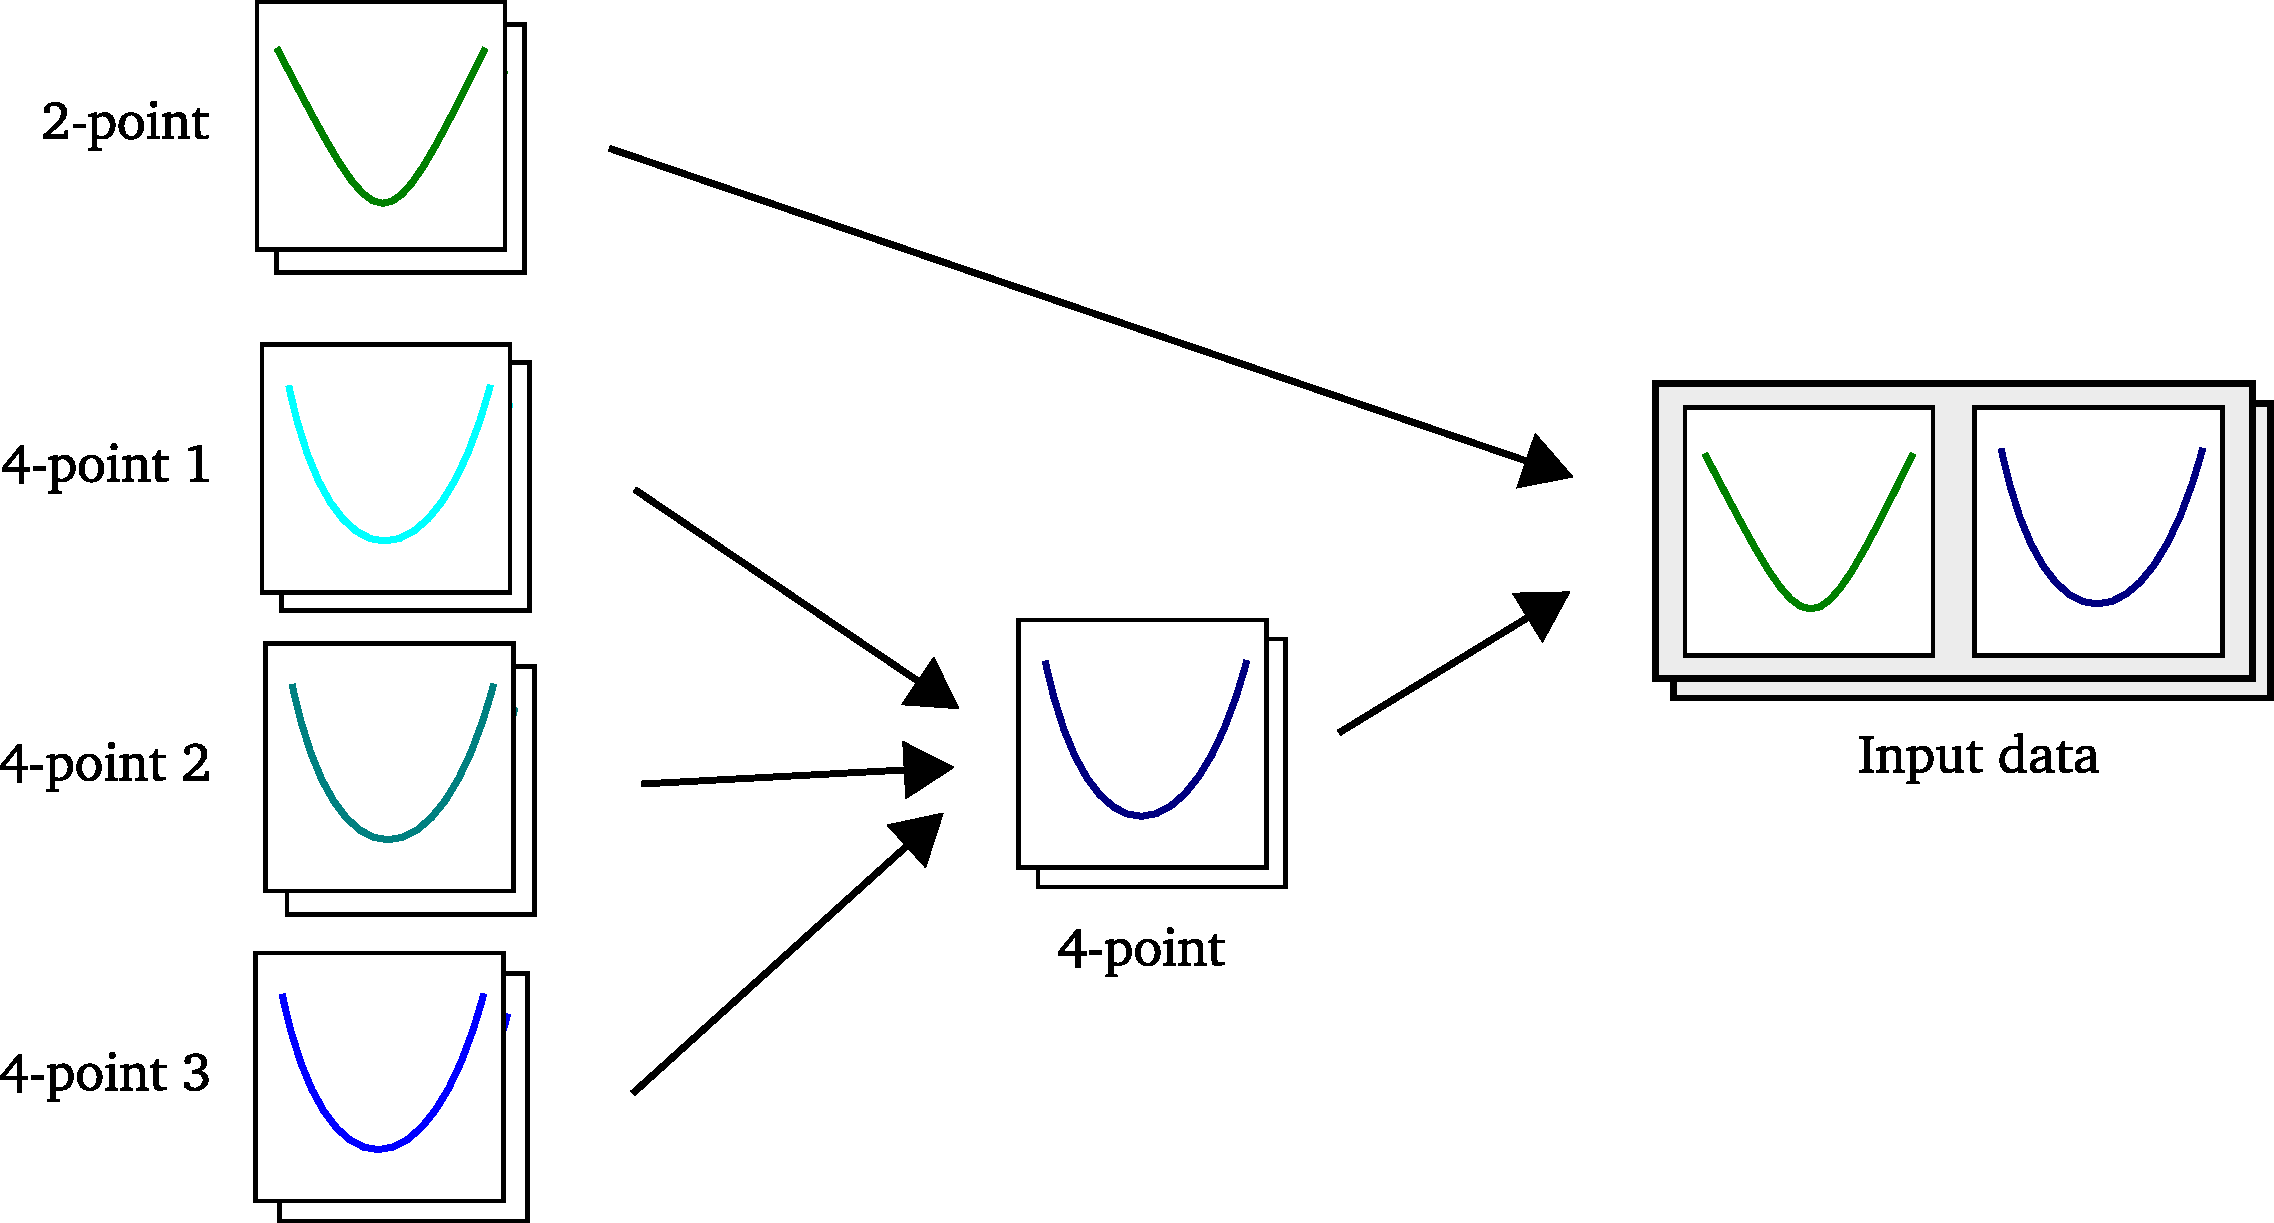
\includegraphics[scale=\scale]{sketches/01-input.pdf}
    \end{center}
\end{frame}

\begin{frame}
    \frametitle{Folding}
    \begin{center}
        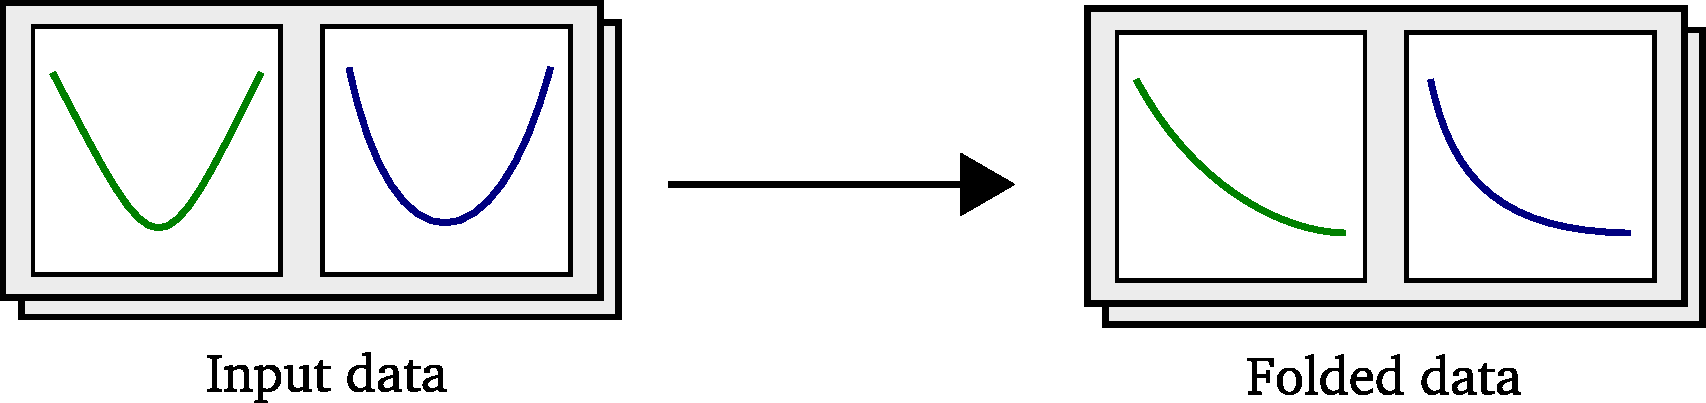
\includegraphics[scale=\scale]{sketches/02-folding.pdf}
    \end{center}
\end{frame}

\subsection{Bootstrap}

\begin{frame}
    \frametitle{Bootstrap}
    \begin{center}
        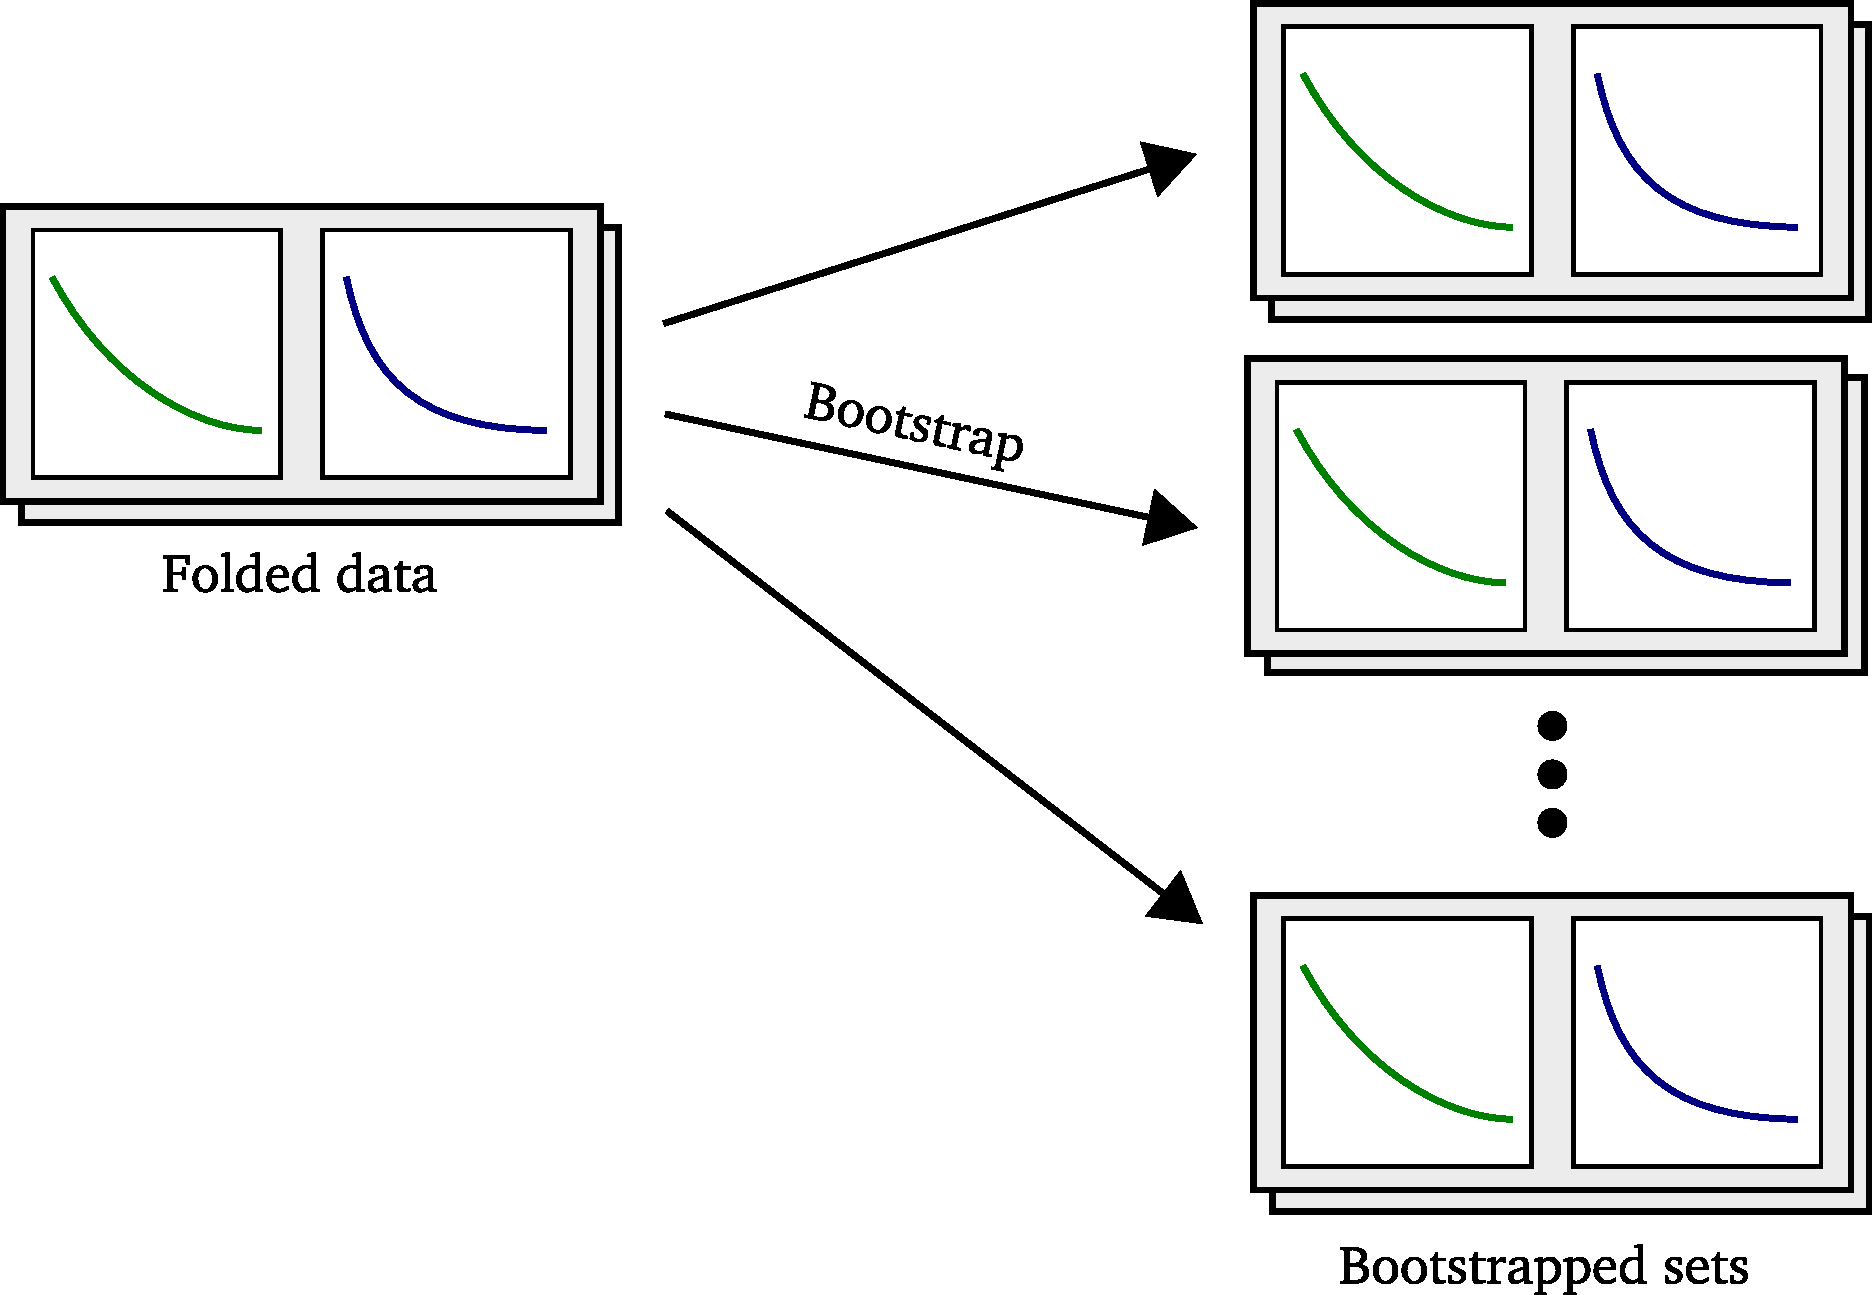
\includegraphics[scale=\scale]{sketches/03-bootstrap.pdf}
    \end{center}
\end{frame}

\begin{frame}
    \frametitle{Bootstrap}
    \begin{center}
        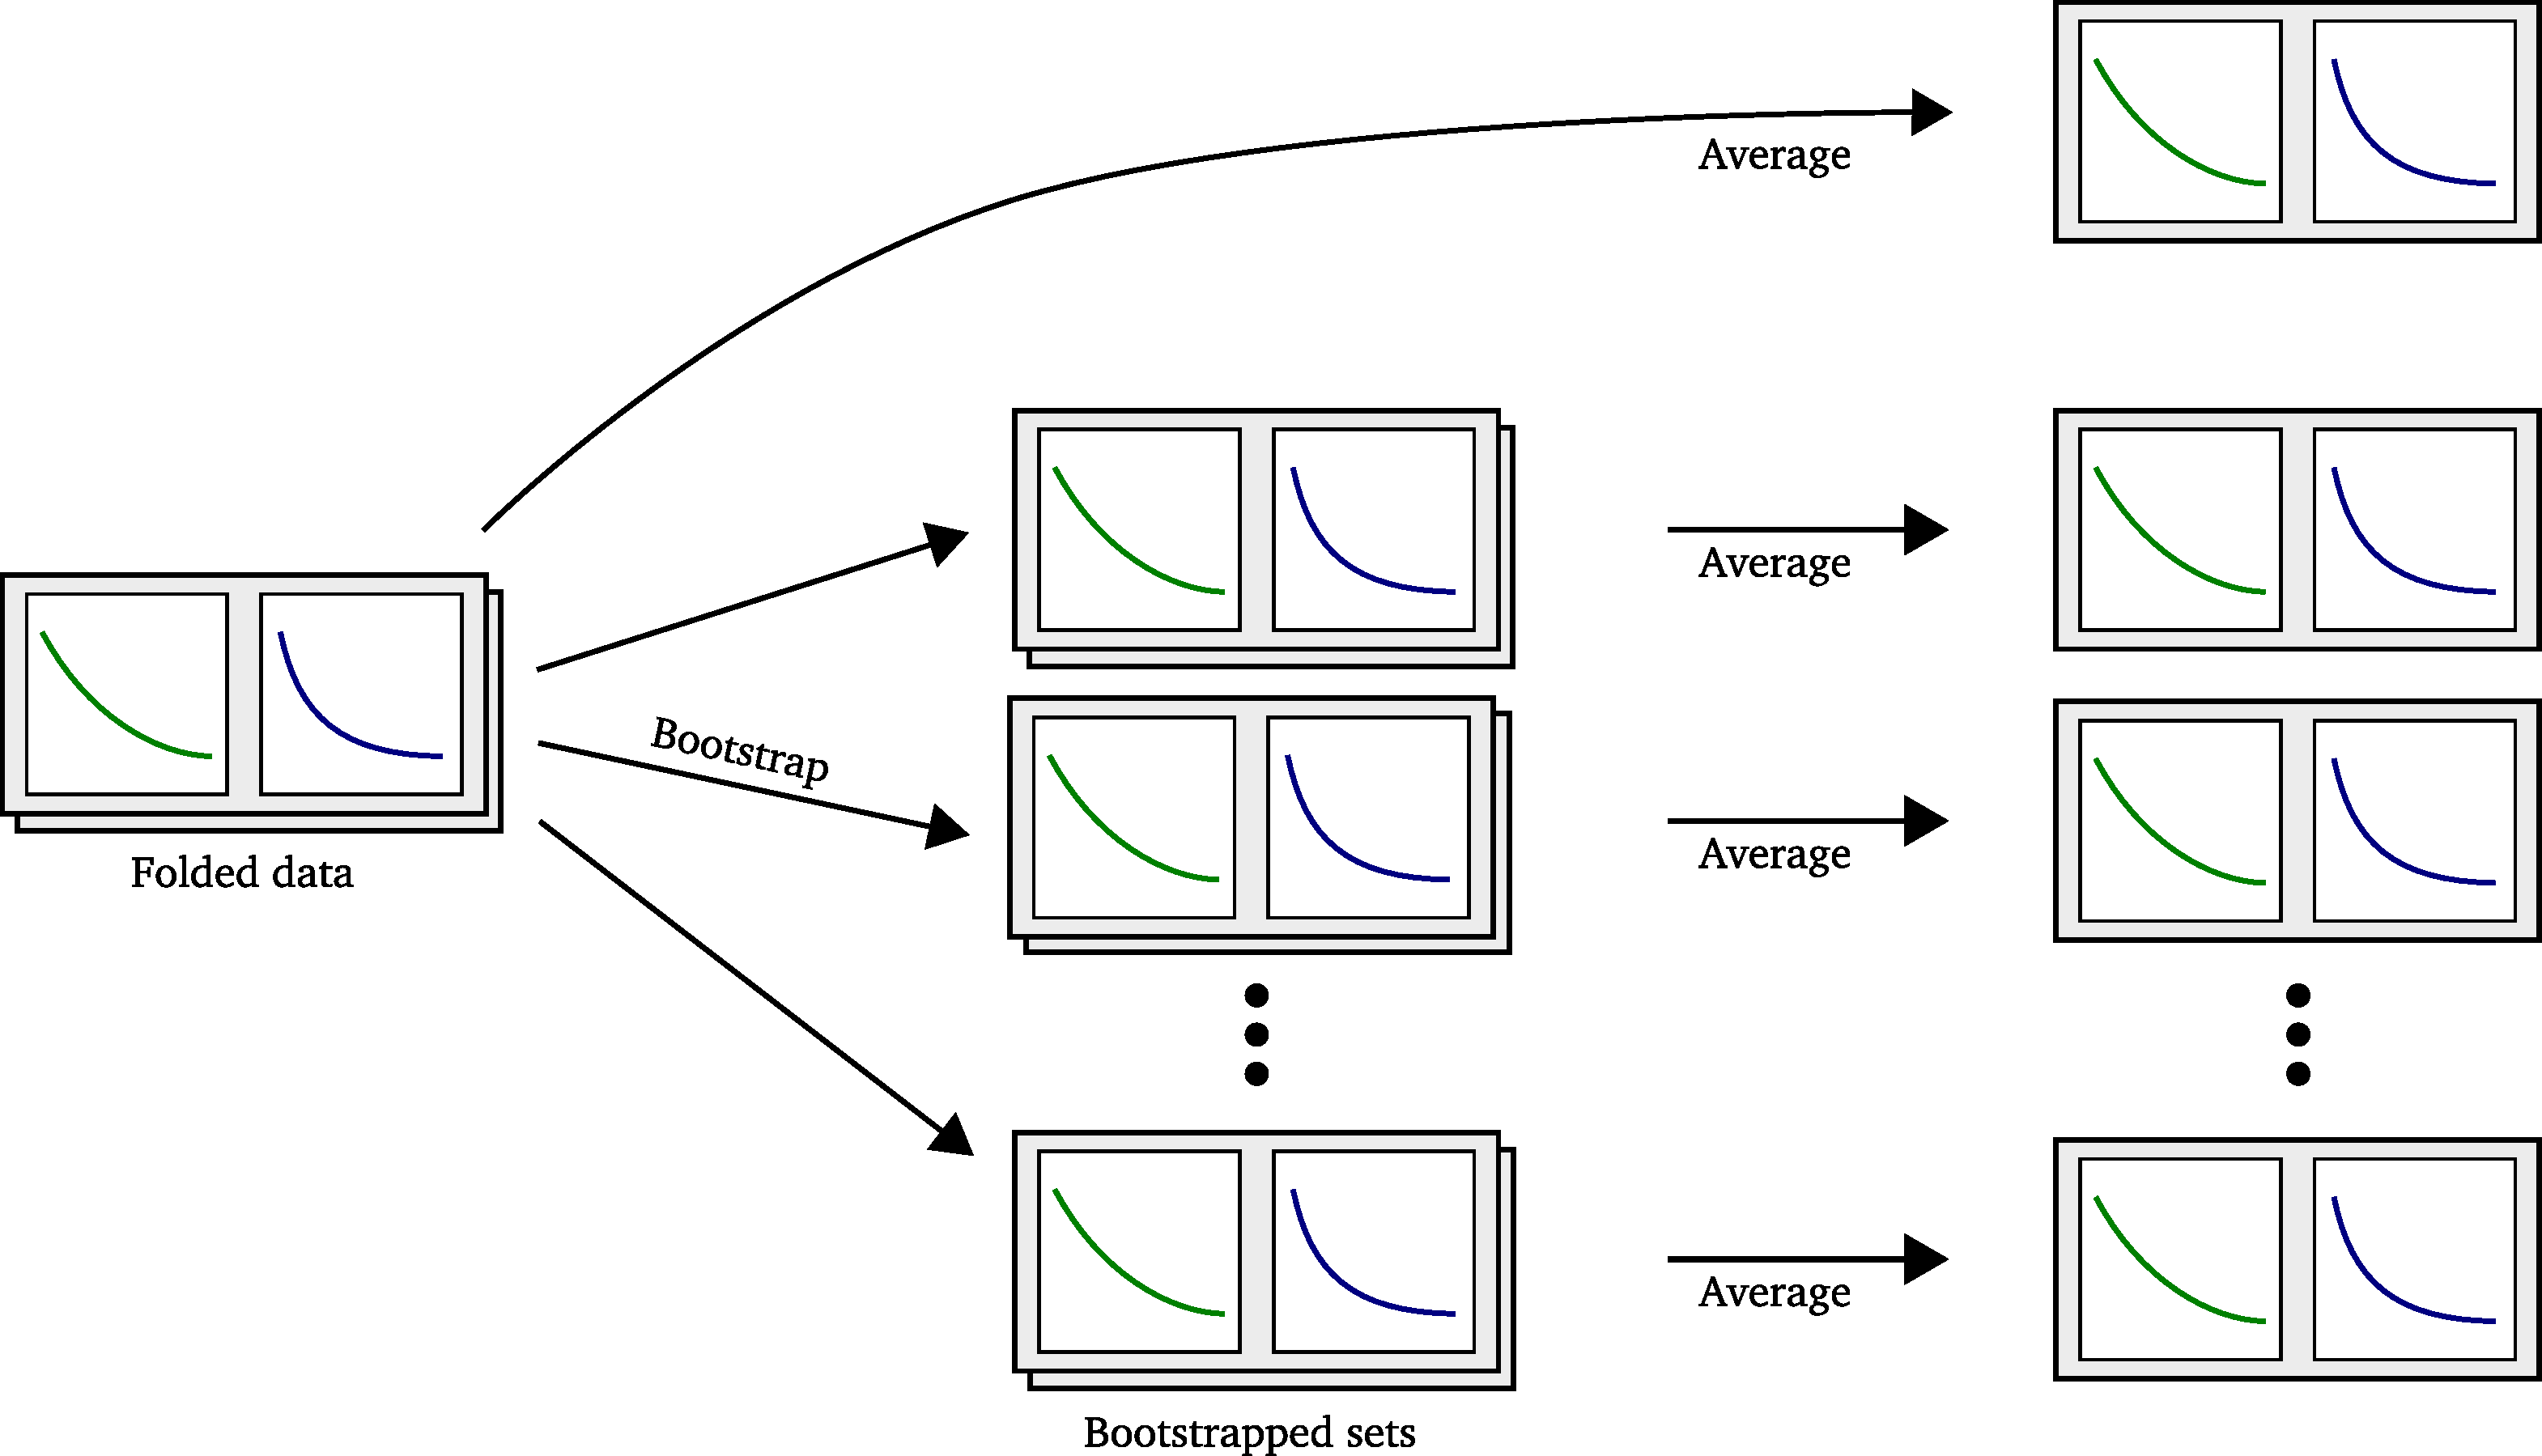
\includegraphics[scale=\scale]{sketches/04-bootstrap.pdf}
    \end{center}
\end{frame}

\subsection{Correlated fit}

\begin{frame}
    \frametitle{Correlation matrix}
    \begin{center}
        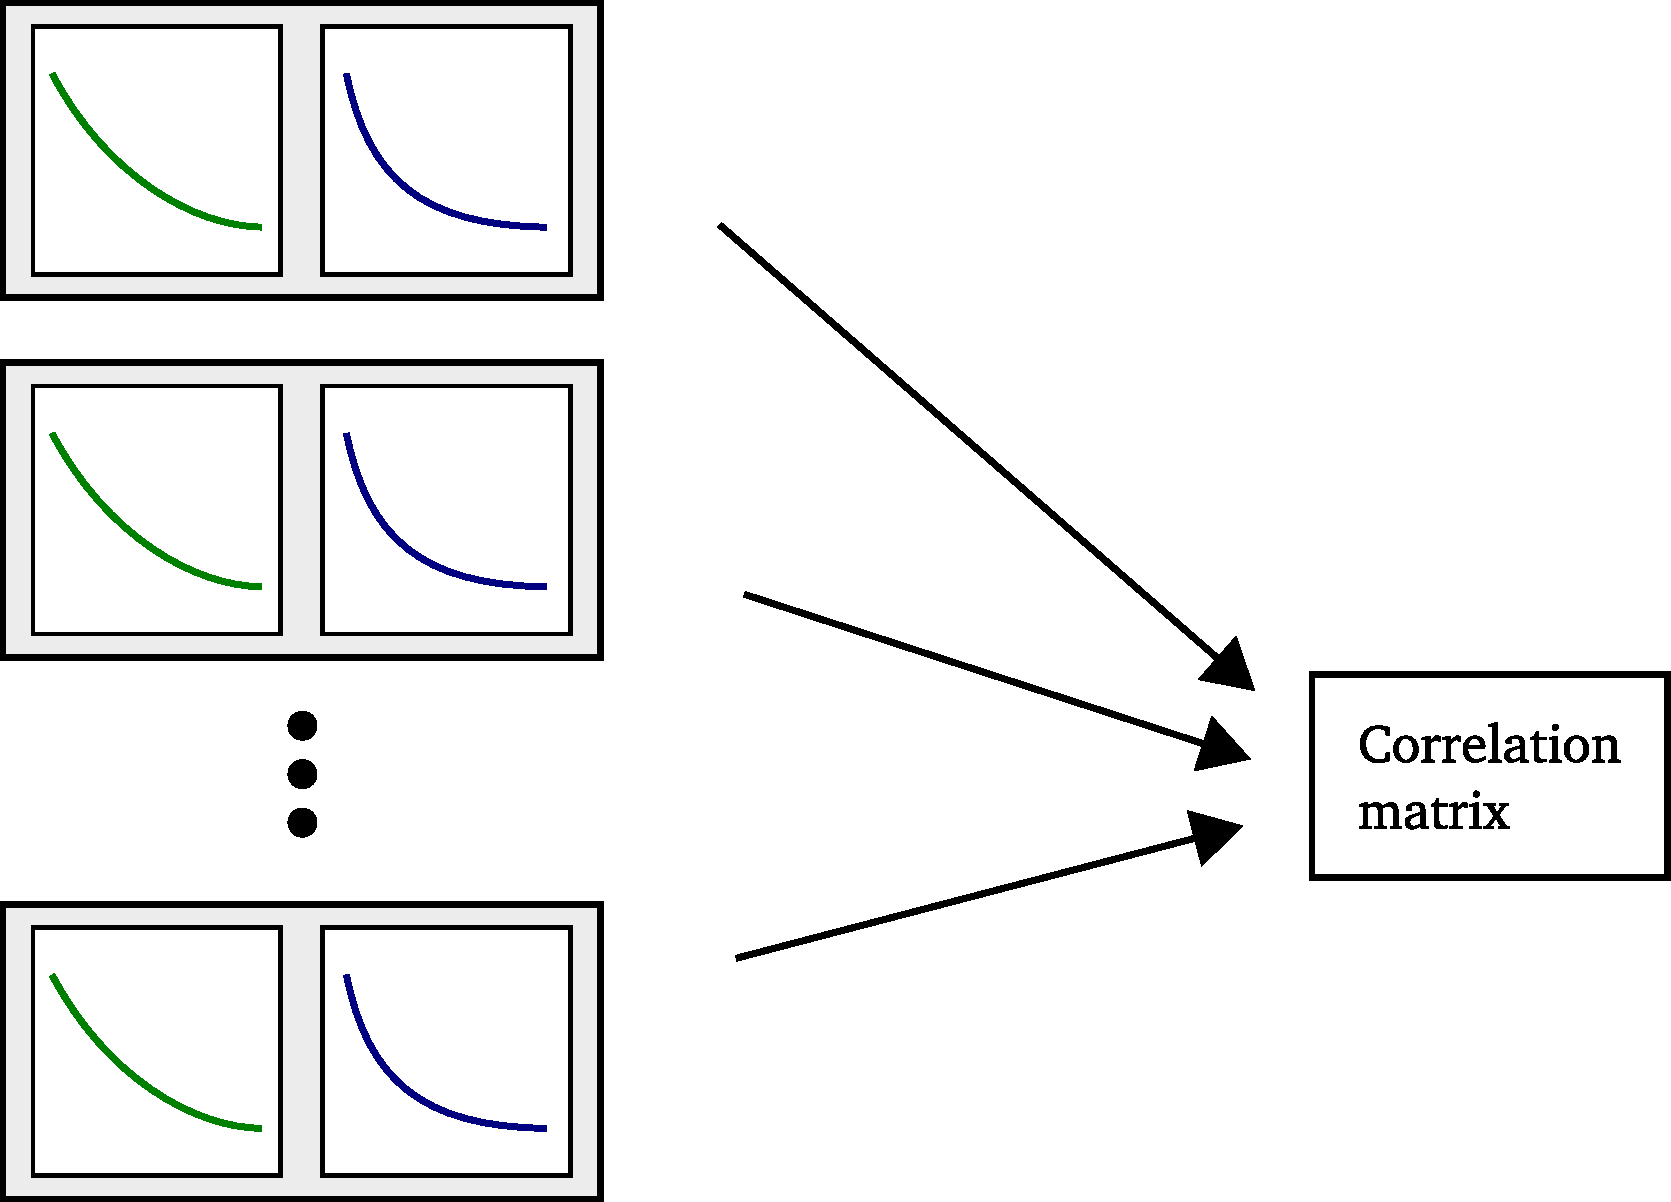
\includegraphics[scale=\scale]{sketches/05-matrix.pdf}
    \end{center}
\end{frame}

\begin{frame}
    \frametitle{Correlated fit}
    \begin{center}
        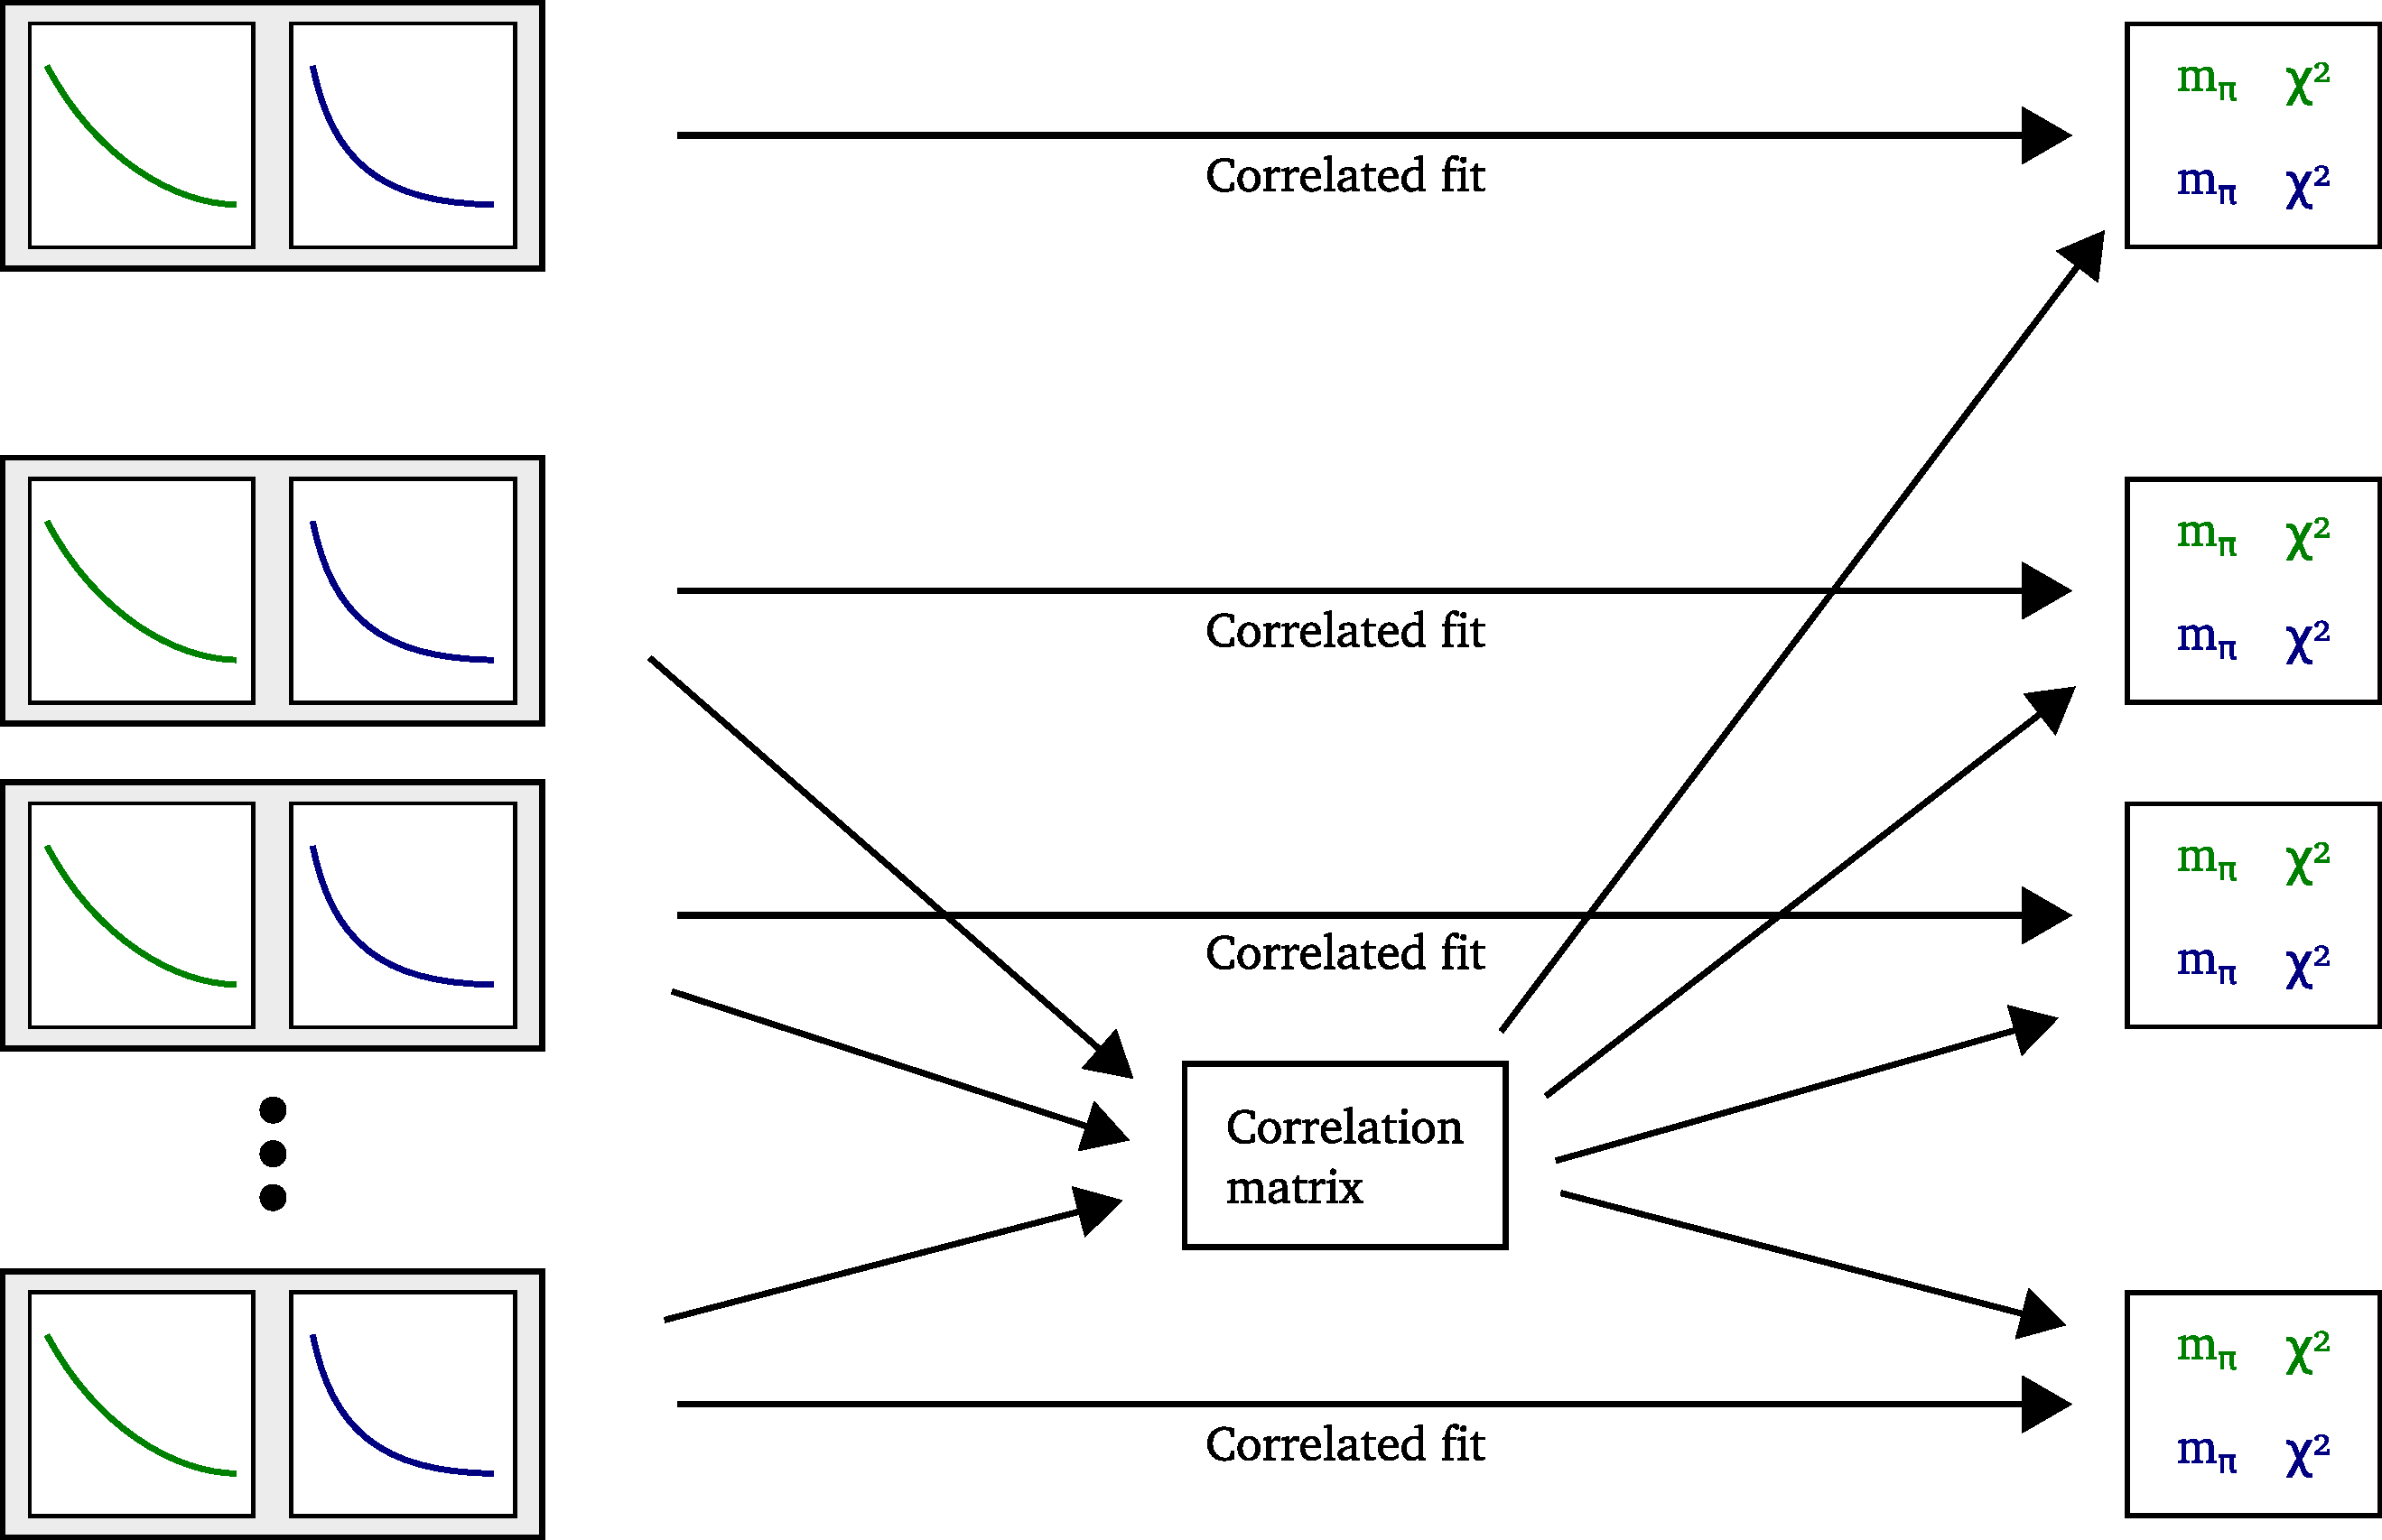
\includegraphics[scale=\scale]{sketches/06-fit.pdf}
    \end{center}
\end{frame}

\subsection{Scattering length}

\begin{frame}
    \frametitle{Lüscher formula}
    \begin{center}
        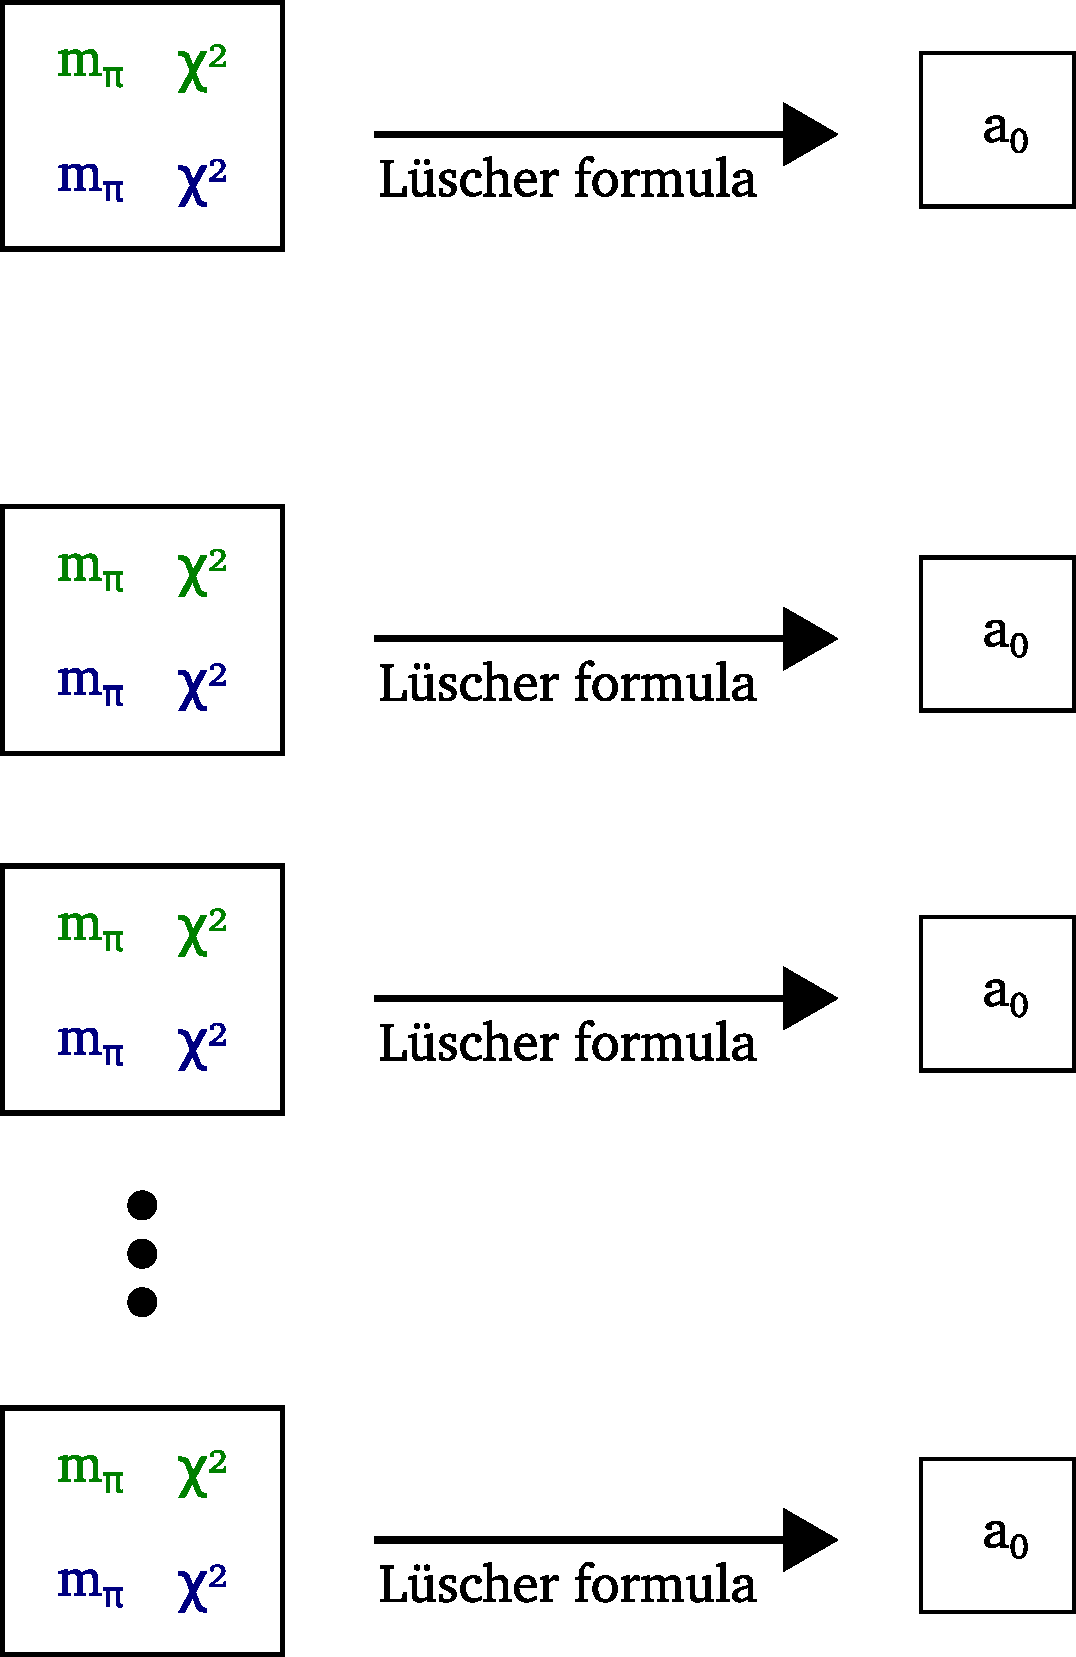
\includegraphics[scale=\scale]{sketches/07-luescher.pdf}
    \end{center}
\end{frame}

\begin{frame}
    \frametitle{End results}
    \begin{center}
        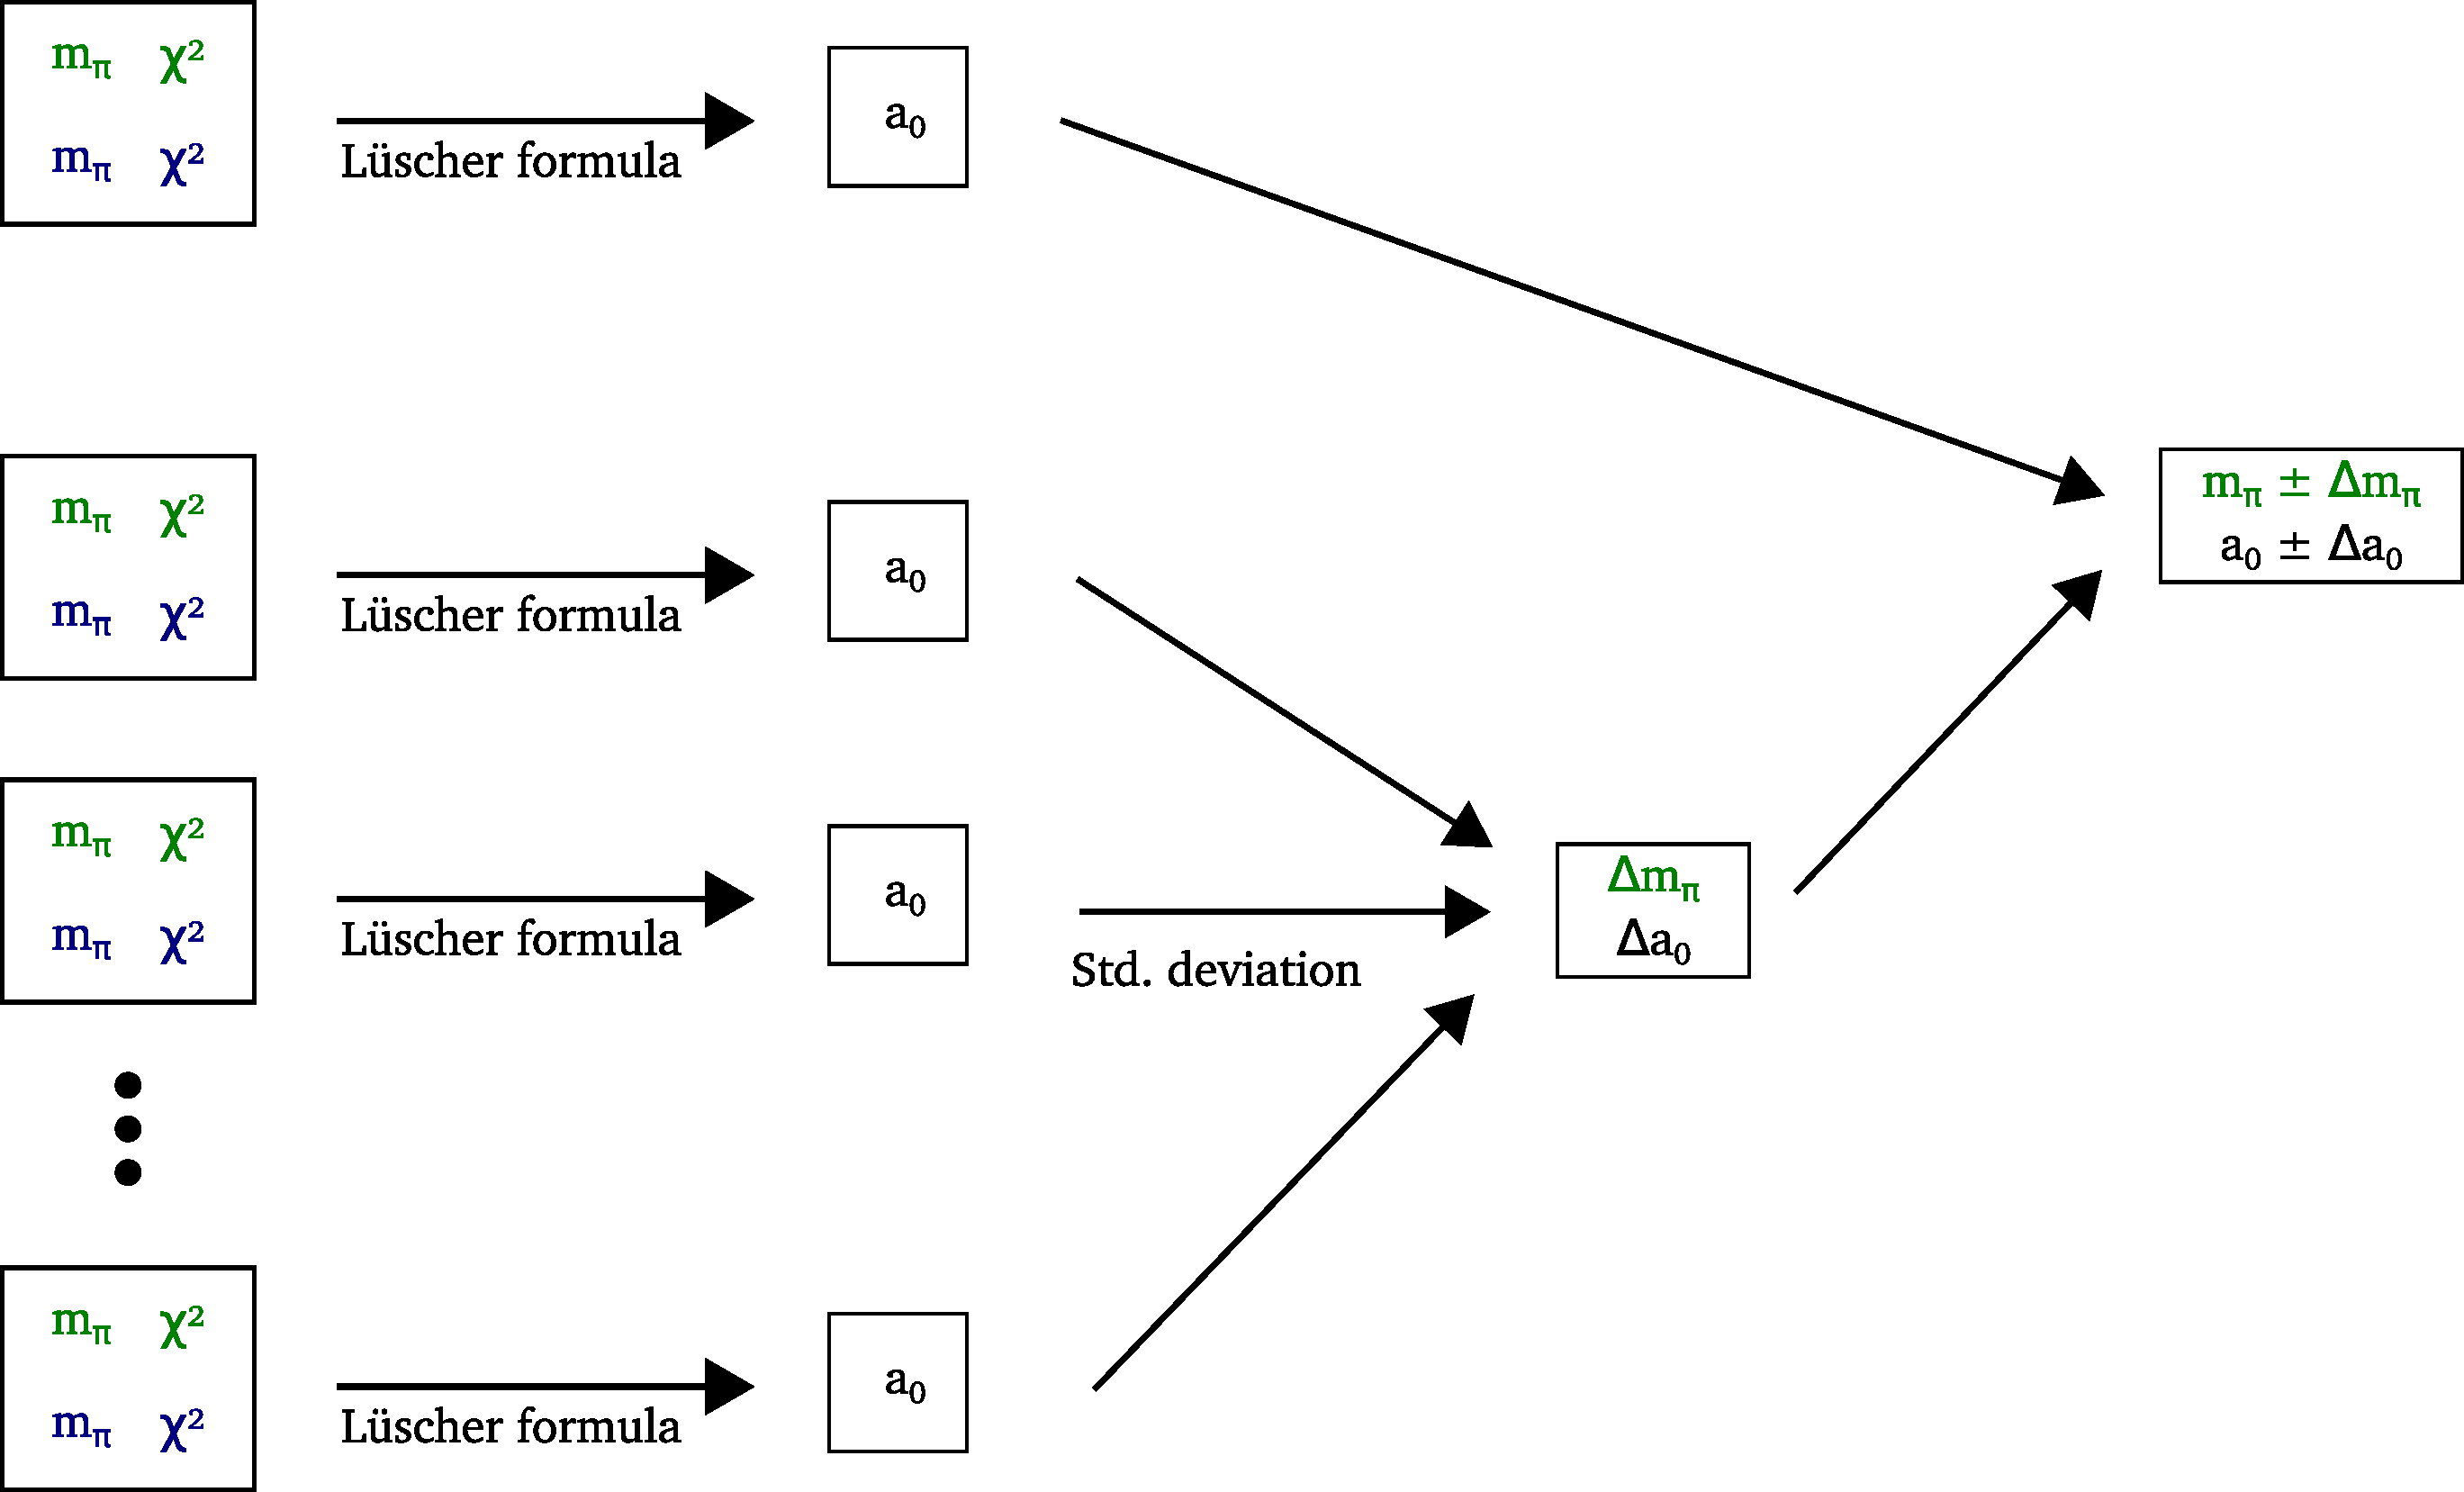
\includegraphics[scale=\scale]{sketches/08-end-result.pdf}
    \end{center}
\end{frame}

%%%%%%%%%%%%%%%%%%%%%%%%%%%%%%%%%%%%%%%%%%%%%%%%%%%%%%%%%%%%%%%%%%%%%%%%%%%%%%%
%                                   Results                                   %
%%%%%%%%%%%%%%%%%%%%%%%%%%%%%%%%%%%%%%%%%%%%%%%%%%%%%%%%%%%%%%%%%%%%%%%%%%%%%%%

\section{Results}

\begin{frame}
    \begin{centering}
        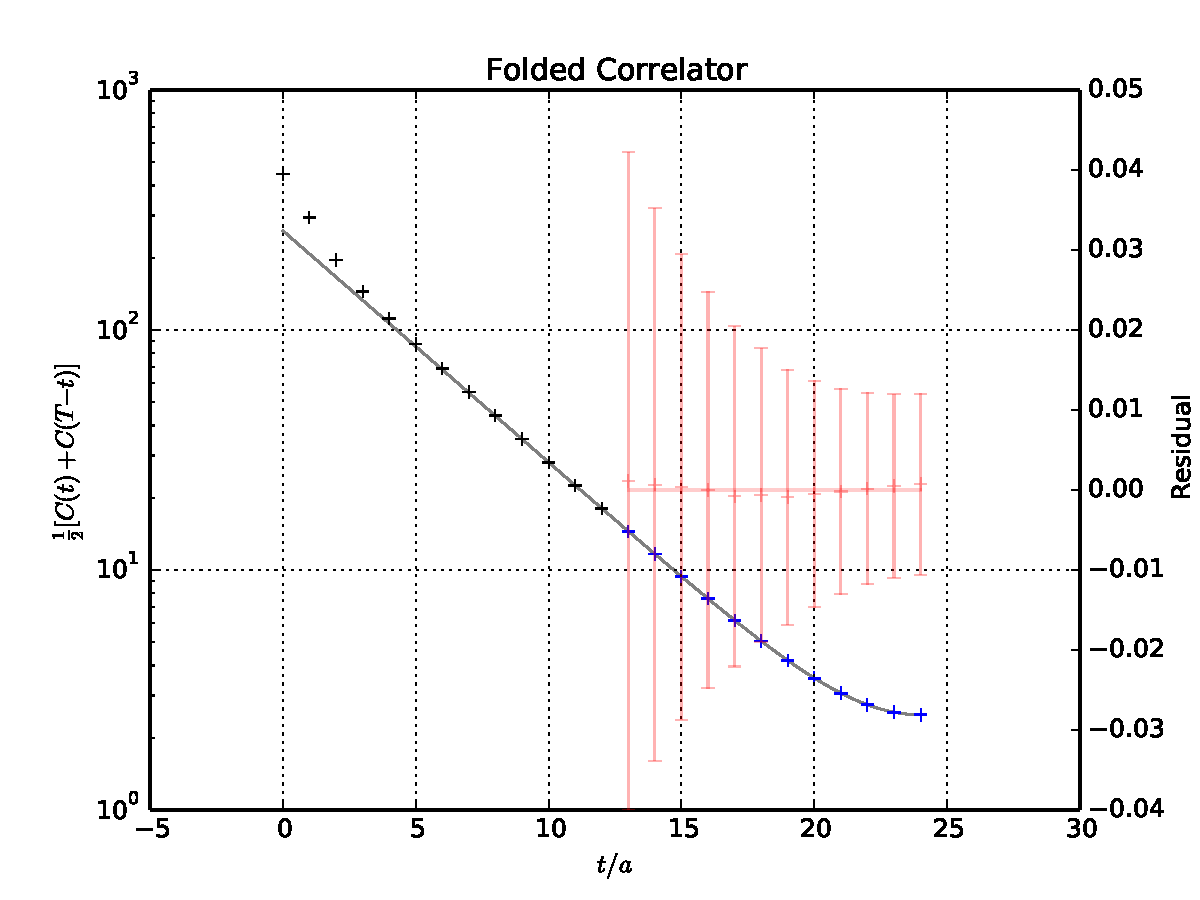
\includegraphics[height=\textheight]{plots/A100_24_L24_T48_beta190_mul0100_musig150_mudel190_kappa1632550__ev120__TB2_SO_LI6_new_c2_folded.pdf}
    \end{centering}
\end{frame}

\begin{frame}
    \begin{centering}
        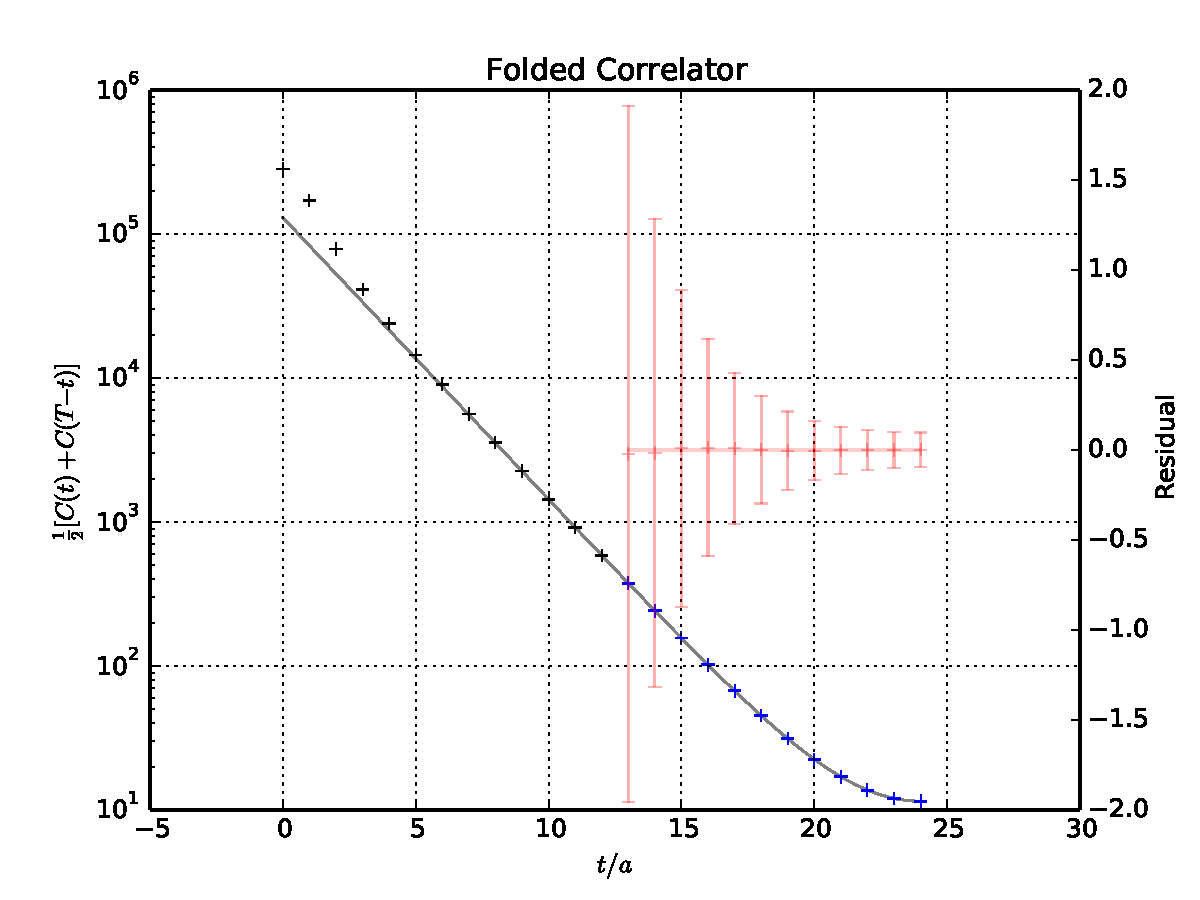
\includegraphics[height=\textheight]{plots/A100_24_L24_T48_beta190_mul0100_musig150_mudel190_kappa1632550__ev120__TB2_SO_LI6_new_c4_folded.pdf}
    \end{centering}
\end{frame}

\begin{frame}
    \begin{centering}
        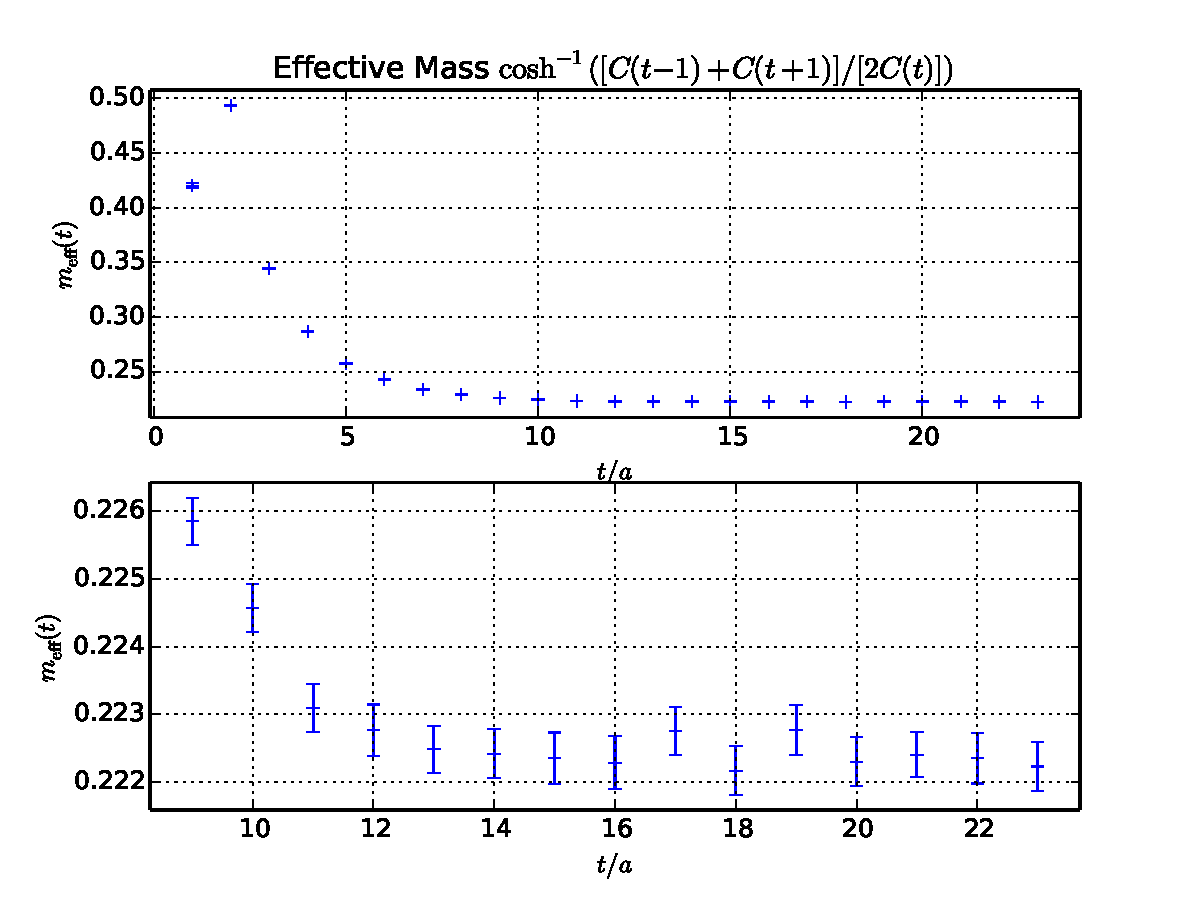
\includegraphics[height=\textheight]{plots/A100_24_L24_T48_beta190_mul0100_musig150_mudel190_kappa1632550__ev120__TB2_SO_LI6_new_c2_m_eff.pdf}
    \end{centering}
\end{frame}

\begin{frame}
    \begin{centering}
        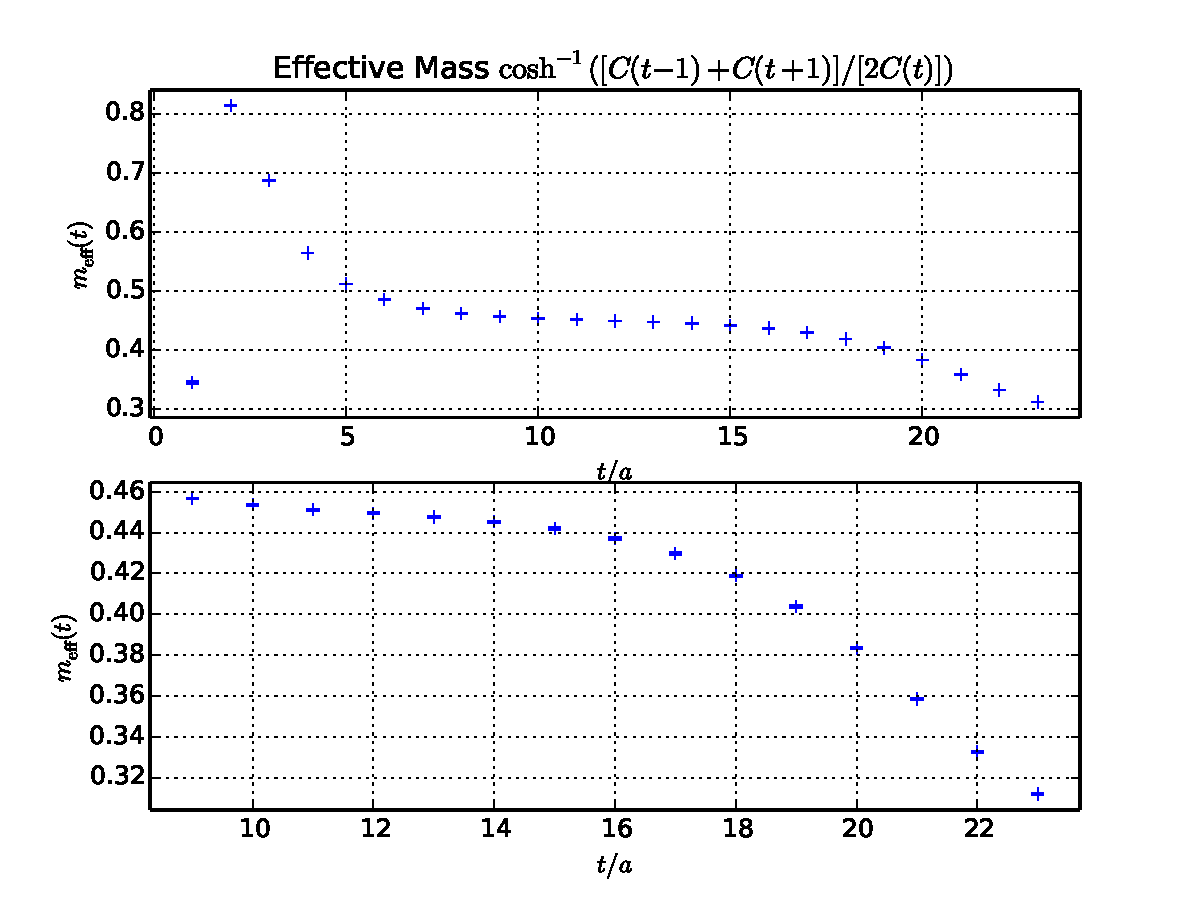
\includegraphics[height=\textheight]{plots/A100_24_L24_T48_beta190_mul0100_musig150_mudel190_kappa1632550__ev120__TB2_SO_LI6_new_c4_m_eff.pdf}
    \end{centering}
\end{frame}

\begin{frame}
    \begin{centering}
        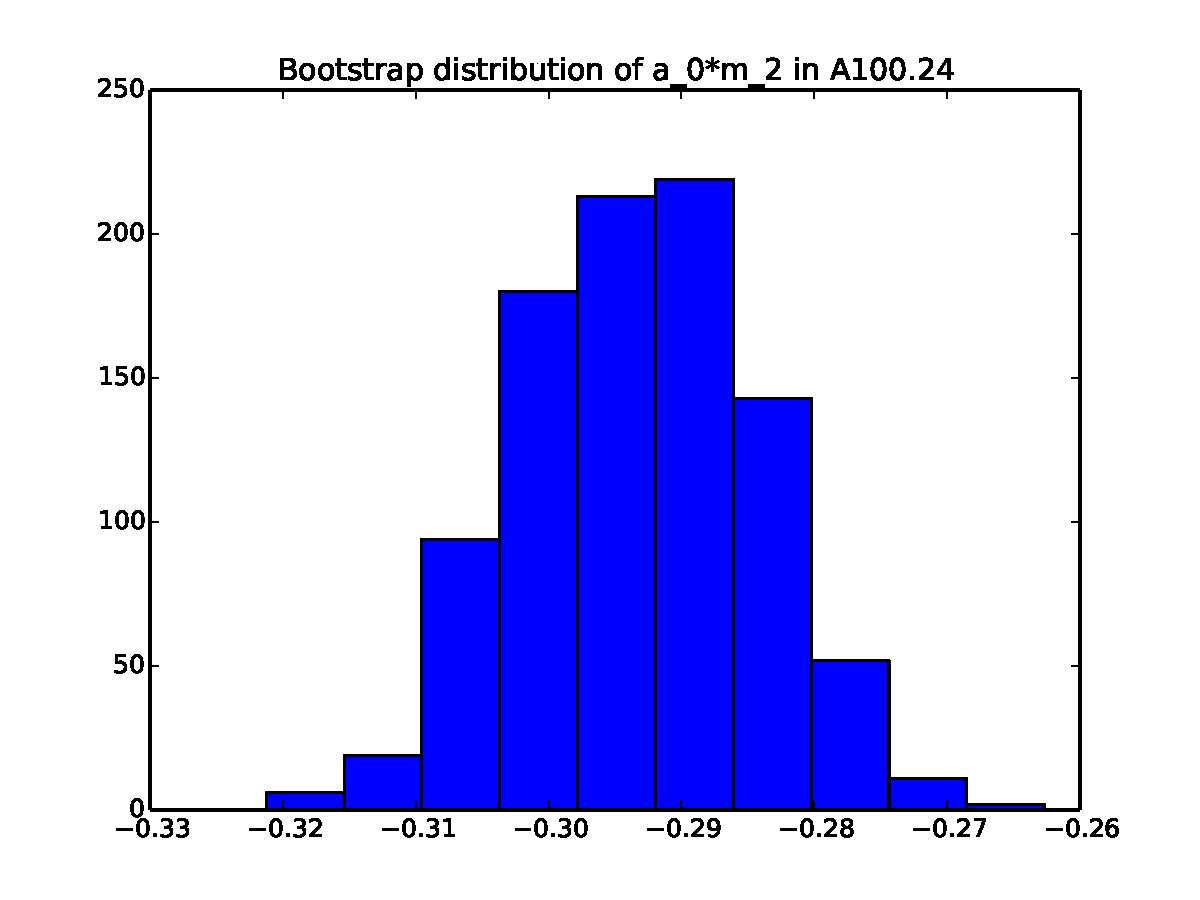
\includegraphics[height=\textheight]{plots/A100_24_L24_T48_beta190_mul0100_musig150_mudel190_kappa1632550__ev120__TB2_SO_LI6_new_boot-hist_a_0*m_2.pdf}
    \end{centering}
\end{frame}

\begin{frame}
    \begin{centering}
        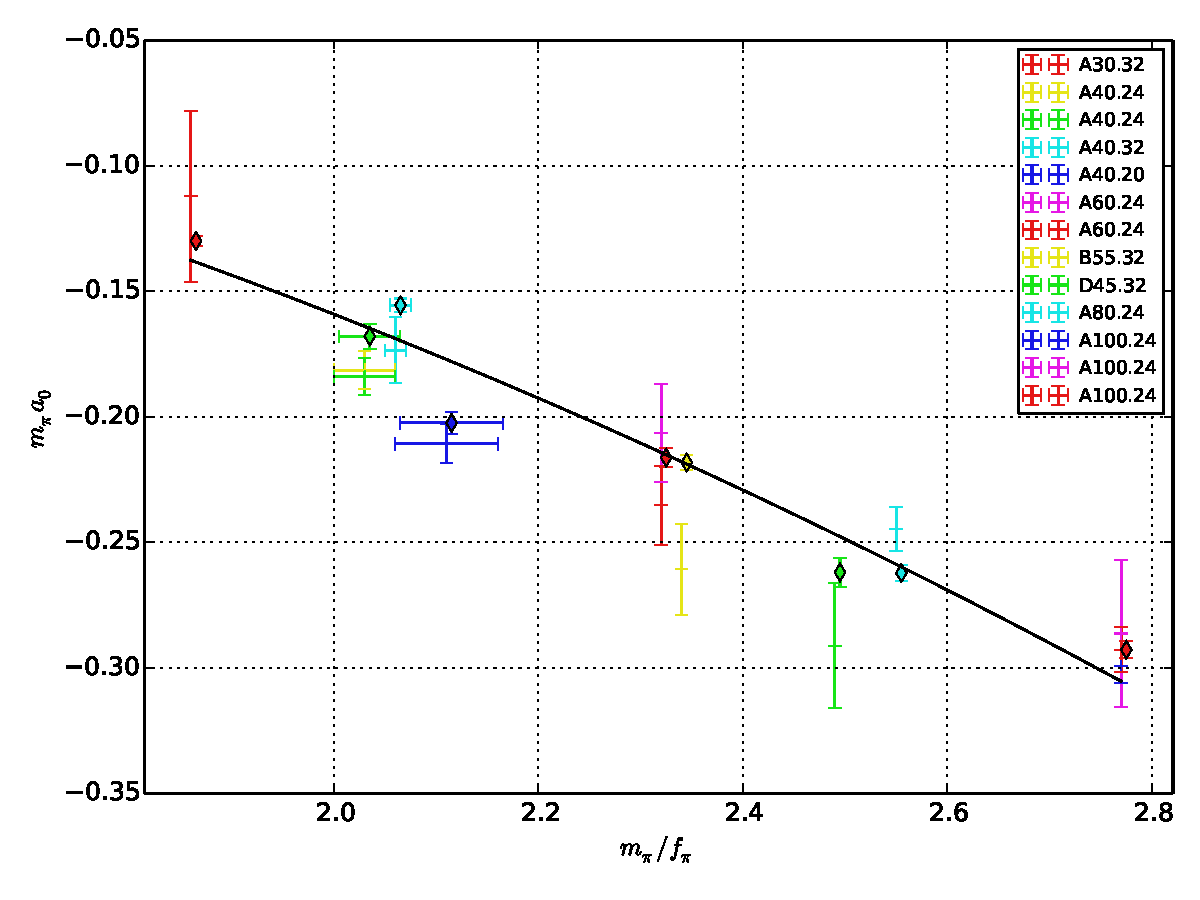
\includegraphics[height=\textheight]{plots/result.pdf}
    \end{centering}
\end{frame}

%%%%%%%%%%%%%%%%%%%%%%%%%%%%%%%%%%%%%%%%%%%%%%%%%%%%%%%%%%%%%%%%%%%%%%%%%%%%%%%
%                                 End matter                                  %
%%%%%%%%%%%%%%%%%%%%%%%%%%%%%%%%%%%%%%%%%%%%%%%%%%%%%%%%%%%%%%%%%%%%%%%%%%%%%%%

\section*{References}

\begin{frame}
    \frametitle{References}

    \printbibliography
\end{frame}

\section*{Download}

\begin{frame}
    \frametitle{Get the paper}

    \begin{columns}[t]
        \begin{column}{0.5\linewidth}
            To get the paper, go to:
            \begin{itemize}
                \item \href{http://martin-ueding.de/en/university/msc_physics/physics760/index.html}{martin-ueding.de}
                \item University
                \item Master of Science in Physics
                \item physics760 Computational Physics
            \end{itemize}
        \end{column}
        \begin{column}{0.5\linewidth}
            Or scan the code:
            \begin{centering}
                
\includegraphics[width=\linewidth]{physics760.png}
            \end{centering}
        \end{column}
    \end{columns}

\end{frame}

\end{document}

% vim: spell spelllang=en
